\aufgabe{PDP and ICE in case of interactions}{

Let us assume that we fitted the following linear regression model with two features: 

\begin{equation}
  \fh(\xv) = \fh(x_1, x_2) = \hat\beta_1 x_1 + \hat\beta_2 x_2 + \hat\beta_3 x_1 x_2 + \hat\beta_0.
  \label{eq:linmod}
\end{equation}


\begin{enumerate}[a)]
  \item Analytically derive the PD function of feature $S = \{1\}$ (with $C = \{2\}$).\\
  \textit{Hint:} In the lecture slides we derived the PD function for a
  linear regression model without an interaction term.\\
  \textit{Hint:} In the end, your solution should include terms like the expected value of $X_2$.
  \item Let us assume that the estimated coefficients in Equation~\ref{eq:linmod}
  are $\hat\beta_0 = 0$, $\hat\beta_1 = -8$, $\hat\beta_2 = 0.2$ and $\hat\beta_3 = 16$.
  Furthermore, $X_1 \sim Unif(-1, 1)$ is uniformly distributed between -1 and 1, 
  and $X_2 \sim B(1, 0.5)$ origins from a Bernoulli distribution. 
  Compute the exact PD function of feature $X_1$ using your derived function of a).
  \item The following plot displays the ICE curves of $X_1$. The rugs show the marginal distribution of $X_1$. 
  Please note that since $X_2$ is binary, we do not receive $n$ individual ICE curves, but indeed 
  only two unique ones. 
  Derive the conditional expectation functions $\fh_1^{(i)}(x_1)$ of $X_1$ for group $X_2 = 1$ and for group $X_2 = 0$ using Equation~\ref{eq:linmod} given the estimated coefficients of b). 
  Which color coding (light green or light blue) reflects the group $X_2 = 1$, which one group $X_2 = 0$?

	\begin{center}
	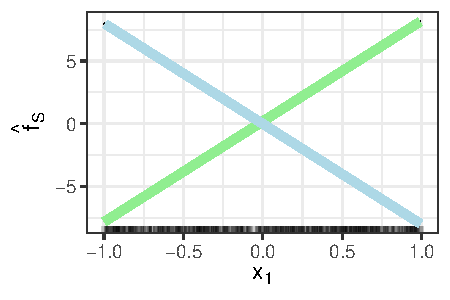
\includegraphics[width=\maxwidth]{figure/pdpinteraction_ICE_curve.pdf} 
	\end{center}

  \item Add the PDP you derived in b) to the plot. 
  Use this example to explain briefly why it is advisable to display not only the PDP but also the ICE curves, 
  when visualizing the feature effects of a specific model. 
\end{enumerate}
}